\documentclass[10pt]{scrartcl}

\usepackage[utf8]{inputenc}
\usepackage{tabularx}
\usepackage{longtable}
\usepackage[ngerman]{babel}
\usepackage[automark]{scrpage2}
\usepackage{amsmath,amssymb,amstext}
%\usepackage{mathtools}
\usepackage[]{color}
\usepackage[]{enumerate}
\usepackage{graphicx}
\usepackage{lastpage}
\usepackage[perpage,para,symbol*]{footmisc}
\usepackage{listings} 
\usepackage[pdfborder={0 0 0},colorlinks=false]{hyperref}
\usepackage[numbers,square]{natbib}
\usepackage{color}
\usepackage{colortbl}
\usepackage[absolute]{textpos}
\usepackage{float}

\lstset{numbers=left, numberstyle=\tiny, numbersep=5pt, breaklines=true, showstringspaces=false} 
\restylefloat{figure}

%changehere
\def\titletext{Praktikum 1 : Modellierung von Raumgestalten}
\def\titletextshort{Praktikum 1}
\author{André Harms, Oliver Steenbuck, Armin Steudte  \\ Carsten Noetzel, Dennis Blauhut, Torben Becker}

\title{\titletext}

%changehere Datum der Übung
\date{26.10.2011}

\pagestyle{scrheadings}
%changehere
\ihead{MI, Thiel-Clemen}
\ifoot{Generiert am:\\ \today}

\cfoot{Oliver Steenbuck, André Harms \\  Armin Steudte, Carsten Noetzel \\ Dennis Blauhut, Torben Becker}


\ohead[]{\titletextshort}
\ofoot[]{{\thepage} / \pageref{LastPage}}

\setlength{\parindent}{0.0in}
\setlength{\parskip}{0.1in}

\begin{document}
\maketitle

\setcounter{tocdepth}{3}
\tableofcontents

	\listoftables                                 												% 
	\listoffigures   

\section{Einleitung}

\section{Räumliche Darstellung}
Zur Modellierung der räumlichen Gegebenheiten am Campus Berliner Tor haben wir ein zweidimensionales Raster gewählt.
In diesem Modell wird der Campus aus Kacheln zusammen gesetzt, bei dem jede Kachel einem bestimmten Geländemerkmal entspricht.
Dieses ermöglicht es die wesentlichen räumlichen Gegebenheiten auf einer höheren Abstraktionsebene darzustellen, so dass der Detailgrad verringert werden kann.\\
Zur Veranschaulichung des Modellierungskonzepts wurde die Abbildung \ref{img:tile_map} mit Hilfe des Tools \textit{Tiled Map Editor} erstellt. Hierbei wurde beispielhaft ein Ausschnitt des Luftbildes des Campus modelliert.
Dieser ist in Abbildung \ref{img:google_maps} gekennzeichnet.\\
Um die verschiedenen Geländemerkmale zu visualisieren, haben wir jeden Geländemerkmal eine Farbe zugeordnet und die jeweiligen Kacheln der Geländemerkmale in dieser Farbe eingefärbt. Die folgende Tabelle gibt eine Übersicht über die verwendeten Farben und die korrespondierenden Merkmale:

\definecolor{gebaude_durchgang}{rgb}{0.341176471,0.780392157,0.945098039}
\definecolor{gebaude}{rgb}{1,0.921568627,0.474509804}
\definecolor{gruenanlage}{rgb}{0.254901961,0.717647059,0.145098039}
\definecolor{hof}{rgb}{0.050980392,0.48627451,0.690196078}
\definecolor{gehweg}{rgb}{0.68627451,0.709803922,0.682352941}
\definecolor{strasse}{rgb}{0.560784314,0.91372549,0.439215686}
\definecolor{gehweg_sek}{rgb}{0.623529412,0.490196078,0.203921569}

\begin{table}[h]	
	\centering
\begin{tabular}{|c|c|}
\hline 
\textbf{Farbe} & \textbf{Geländemerkmal} \\ 
\hline 
\cellcolor{gebaude} & Gebäude \\
\hline 
\cellcolor{gebaude_durchgang} & Gebäudedurchgang\\
\hline 
\cellcolor{gruenanlage} &  Grünanlage\\ 
\hline 
\cellcolor{hof} &  Hof\\ 
\hline 
\cellcolor{gehweg} & Gehweg\\ 
\hline 
\cellcolor{gehweg_sek} & Sekundär Gehweg\\
\hline 
\cellcolor{strasse} & Straße\\ 
\hline 
\end{tabular} 
	\label{tab:colorMap}
	\caption{Farbbedeutungen in der räumlichen Darstellung}	
\end{table}	



        
	\begin{figure}[H]
        
                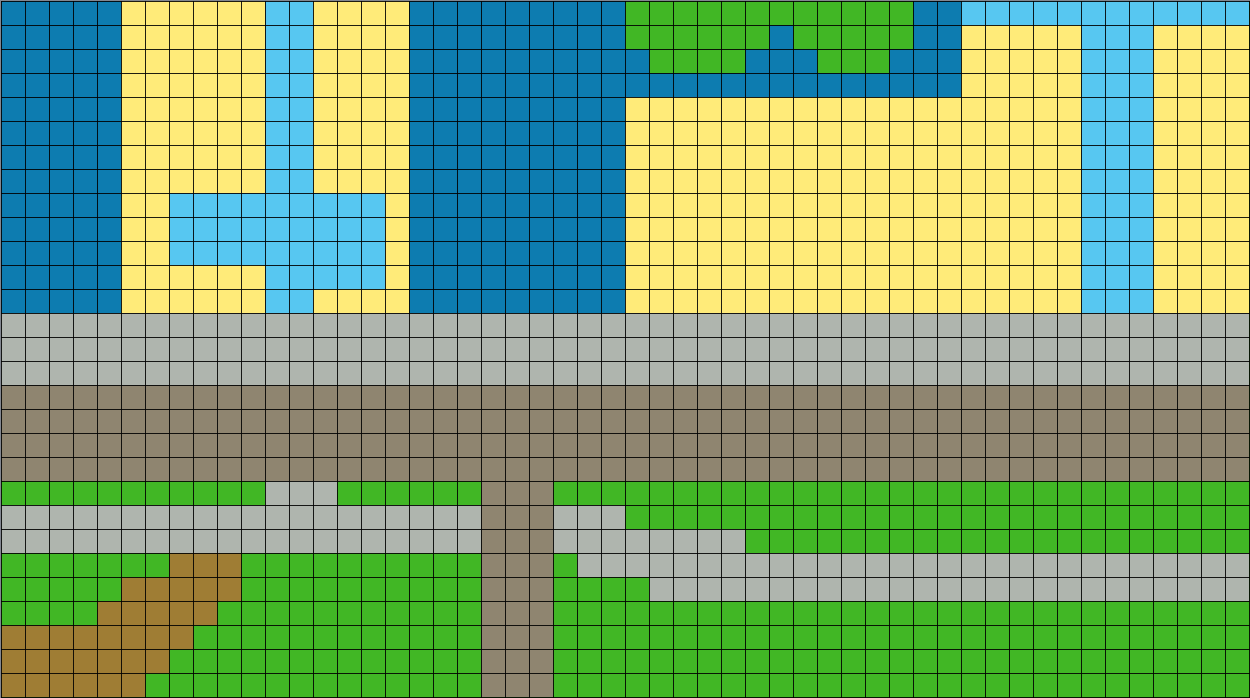
\includegraphics[width=\textwidth]{img/tile_map_campus_pic}
        \caption{Ausschnitt von Campus als \glqq Tilebased Map\grqq{}}
        \label{img:tile_map}
	\end{figure}                
        
	\begin{figure}[H]
        \centering
                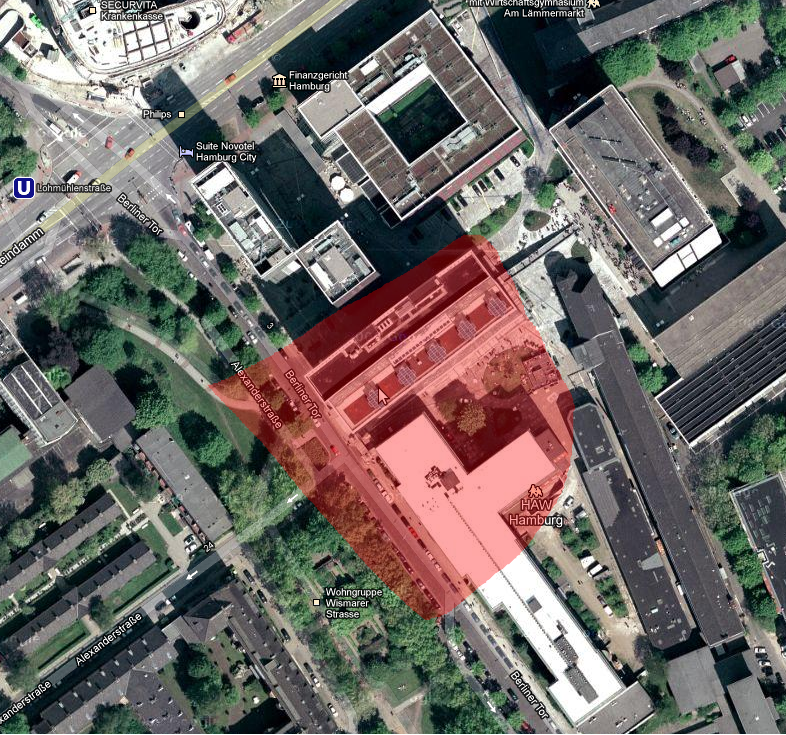
\includegraphics[width=\textwidth]{img/google_maps}
        \caption{Ausschnitt Google-Maps}
        \label{img:google_maps}
	\end{figure}         
  
        
        
        Um andere Aspekte als die räumlichen Gegebenheiten modellieren zu können, ist es möglich ein Ebenenkonzept zu verwenden. Hierbei werden die gewünschten Eigenschaften auf anderen Schichten modelliert. Diese Schichten lassen sich dann entsprechend verwenden und auswerten (vgl. Abschnitt \ref{sec:Ebenen}).
Sollte sich im Verlauf der Praktika herausstellen, dass eine dreidimensionale Modellierung besser geeignet ist, besteht die Möglichkeit, zu einem dreidimensionalem Modell zu wechseln. Hier werden zusätzliche Eigenschaften nicht mehr in Ebenen modelliert sondern in parallelen Räumen, sogenannte \textit{Spaces}.

\section{Entitäten}

	\subsection{Beschreibungen}
	Nachfolgend folgen die Beschreibungen der einzelen Entitäten. Diese sind zur besseren Übersicht in drei Gruppen untergliedert. Die Gruppe \verb!Verkehr! enthält alle diejenigen Entitäten, die zur Modellierung des Verkehrsflusses auf dem Campus genutzt werden. Dabei ist mit Verkehr, sowohl der Fußgängerverkehr, als auch der Kraftverkehr gemeint.
	Die Gruppe \verb!Inventar! hingegen, enthält alle diejenigen Entitäten die auf dem Campusgelände bewegt werden können. Die letzte Gruppe, \verb!Architektur! beinhaltet Entitäten die feste Strukturen darstellen und nicht beweglich sind.\\
	Allen Entitäten leiten von der Klasse \verb!Object! ab und haben damit eine Positon auf dem Campusgelände sowie eine Dimension, die ihre Größe angibt. Jedem Objekt sind Einflussfaktoren zugeordnet, aus denen Metaebene des Modells algorithmisch abgeleitet wird. Dies sind \verb!Vergnügen!,
	\verb!Sozialisierung!, \verb!Sicherheit! und \verb!Produktivität! diese sind im Detail in Abschnitt \ref{sec:Ebenen} beschrieben.
	
	\subsubsection{Verkehr}
	
	

\begin{table}[!htb]
	\centering
\begin{longtable}{|p{0.25\textwidth}|p{0.75\textwidth}|}
\hline \textbf{Entität} & \textbf{Beschreibung} \\ 
\hline
\hline Grünfläche & Parkähnliche in der Regel mit Gras bewachsene Fläche, z.B. zwichen BT5 und Stiftstraße. Andere Entitäten können auf der Grünfläche plaziert werden (z.B. Wege) \\ 
\hline Wege & Repräsentiert einen Fuß oder Radweg mit einer bestimmten Beschaffenheit\\ 
\hline Parkplätze & Eine Anzahl von Parkplätzen für Autos\\ 
\hline Fahrradstellplätze & Eine Anzahl von Stellplätzen für Fahrräder \\ 
\hline Verkehrszeichen & Ein Zeichen zur Verkehrsregelung, z.B. 'Geschwindigkeit 30' \\ 
\hline Ampel & Eine Lichtsignalanlage zur Verkehrsregelung  \\ 
\hline 
\end{longtable}	
	\label{tab:entitiesTraffic}
	\caption{Entitätsliste: Verkehr}	
\end{table}		

\clearpage

\subsubsection{Inventar}	

\begin{table}[!htb]	
	\centering
\begin{longtable}{|p{0.25\textwidth}|p{0.75\textwidth}|}
\hline \textbf{Entität} & \textbf{Beschreibung} \\
\hline
\hline Beleuchtungsquelle & Eine Lichtquelle, die in der Regel halbfest montiert ist \\ 
\hline Bank & Bittet Platz für eine Anzahl \verb!n! von Personen \\ 
\hline Aschenbecher & Aschenbecher führen in de Regel zu Menschenansammlungen \\ 
\hline Mülleimer & Führen direkt um sie herum zu seiner verschmutzen Umgebung, dafür aber in einiger Entfernung zu Sauberkeit\\ 
\hline WLAN AP & Strahlt in einem bestimmten Radius WLAN aus das die Produktivität erhöht\\ 
\hline 
\end{longtable}
	\label{tab:entitiesInventory}
	\caption{Entitätsliste: Inventar}	
\end{table}	

\subsubsection{Architektur}

\begin{table}[!htb]	
	\centering
\begin{longtable}{|p{0.25\textwidth}|p{0.75\textwidth}|}
\hline \textbf{Entität} & \textbf{Beschreibung} \\
\hline	
\hline Gebäude & Eine Gebäude des Campus\\ 
\hline Mauer & Eine freistehende oder in ein Gebäude integrierte Mauer die unter anderem den WLAN Empfang beschränkt\\ 
\hline Eingang & Eingang in ein Gebäude \\ 
\hline Abwasserschacht & z.B. zwischen BT5 und BT21 \\ 
\hline 
\end{longtable}
	\label{tab:entitiesArchitecture}
	\caption{Entitätsliste: Architektur}	
\end{table}	

	\subsection{Klassendiagramm}
	Im folgenden wird das sich aus der vorhergehenden Sektion ergebende Klassendiagramm visualisiert (hier mit VisualParadigm).
	Hier wurde, zum Zweck der Übersichtlichkeit darauf verzichtet darzustellen, dass alle Entitäten von \verb!Objekt! ableiten.
	
	\begin{figure}[H]
    	\label{fig:fachlichesDatenmodellUebersicht}
			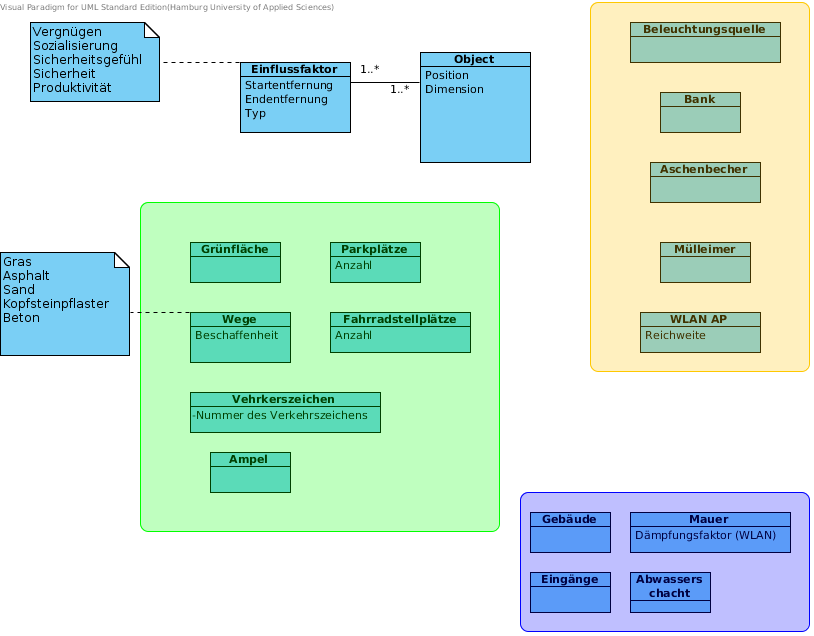
\includegraphics[width=\textwidth]{img/ClassDiagram.png}
            \caption{Klassendiagramm}
             \label{img:classDiagram}
	\end{figure} 	
	
\section{Ebenen}\label{sec:Ebenen}
Eine Ebene ist eine Abstrahierung von Messungen, gefühlten Werten bzw. Erfahrungswerten. Diese Werte werden auf einer Karte in Zonen dargestellt. Eine Zone besteht dabei aus mehreren quadratischen Feldern in der räumlichen Darstellung. Dabei ist der Wert in der Mitte der Zone am höchsten und flacht zum Rand der Zone hin ab. Eine Alternative wäre, dass ein Wert pro Feld dargestellt wird.
\newline Der Wert eines Feldes wird im prozentualen Anteil des maximal möglichen Wertes angegeben und dem entsprechend mit einer Farbe verbunden, die anzeigt, ob etwas gut oder schlecht ist. Als Beispiel die Sicherheit, die auf einer Wiese deutlich höher sein dürfte und grün eingefärbt wäre, als auf einer sechs spurigen Straße in einer Großstadt, die als farbliche Markierung rot wäre.

\subsection{Sicherheit}
Die Sicherheitsebene vergibt Werte für einzelne Bereiche in der räumlichen Darstellung. Eine farbliche Darstellung der einzelnen Bereiche steht für den dahinter liegenden Wert. Je röter der Bereich ist, desto gefährlicher ist es. Und je grüner es wird, um so sicherer fühlen sich Menschen. Dabei steigt zum Beispiel das Gefühl der Sicherheit, je weiter man sich von der Straße fortbewegt oder auf der Straße, wenn mittels eines Zebrastreifens für eine Erhöhung der Sicherheit gesorgt wird.
\newline Es wäre auch möglich, diese Ebene in zwei weitere Ebenen zu unterteilen. Zum einen die gefühlte Sicherheit, die z.B. steigt, wenn Kameras installiert werden und die tatsächliche Sicherheit, die steigt, wenn diese Kameras auch rund um die Uhr überwacht werden und sofort eingeschritten wird und nicht erst zu Hilfe gezogen werden, wenn die Tat bereits passiert ist. Dies ist allerdings ein Schritt, der sich erst in der späteren Modellierung beweisen muss.
\newline Die Sicherheit kann direkten Einfluss nehmen auf das Wohlbefinden der Personen. Denn trotz eines guten Wohlbefindens, kann dieses gemindert werden, wenn die Sicherheit sinkt, indem eine kritische Situation entsteht.

\subsection{Vergnügen}
In der Vergnügen-Ebene wird das Befinden der Personen dargestellt. Auch in dieser Ebene wird die gleiche farbliche Gestaltung verwendet. Ist ein Bereich grün bzw. wird grüner, fühlt sich die Person umso wohler. Ist der Bereich rot resp. wird röter, fühlt sich die Person unwohler. Das Wohlbefinden einer Person kann von unterschiedlichen Faktoren beeinflusst werden, wie z.B. die Nähe zur Straße, Anzahl der Fahrzeuge auf der Straße oder von vorhandenen Grünflächen bzw. Aufenthaltsbereichen mit oder ohne Sitzgelegenheiten.

\subsection{Soziologie}
Mittels der Ebene der Soziologie wird das Empfinden der Menschen zu anderen Menschen dargestellt. Es ist bekannt, dass sich in gewissen Situationen Menschen unwohler fühlen, je enger sie zusammen stehen. Dieses Verhalten lässt sie auf einer Karte gut erkennen. Kleine Gassen bzw. enge Wege oder enge Räume können unbehagen auslösen und werden deshalb rot markiert, während recht große Wege und freie Flächen grün markiert werden.
\newline Dabei soll diese Ebene auch das Verhalten auf Sitzflächen darstellen können. Sich fremde Menschen mögen es nicht, dicht auf einer Parkbank zu sitzen. Anders sieht die Situation wieder mit bekannten Menschen aus, wo dies durchaus angenehm bzw. geduldet wird.
\newline Diese Ebene kann direkten Einfluss auf die Ebenen Sicherheit und Vergnügen nehmen. Denn das Gefühl der Sicherheit kann steigen, wenn man mit bekannten Personen zusammen ist und sinken, je mehr unbekannte Personen um einen herum stehen. Genauso kann auch das Vergnügen steigen und sinken.

%\subsection{Durchfluss}
%In dieser Ebene wird der maximal m\"ogliche Durchfluss eines gewissen Bereiches dargestellt. Es wird eine farbliche Darstellung gew\"ahlt, bei der gr\"un bedeutet, dass viele Personen pro Zeit diesen Bereich passieren k\"onnen respektive rot, wenn eher wenig Personen pro Zeit den Bereich durchqueren k\"onnen.
%\newline Die Erfahrungen bzw. Erkenntnisse dieser Ebene k\"onnen auch direkten Einfluss auf die Feel Good- und Sicherheitsebene haben. Ist an einer gewissen Stelle der Karte der maximal m\"ogliche Durchfluss gering und es ist bekannt, dass zu gewissen Zeiten aber viele Menschen durch diesen Bereich wollen, k\"onnte dies einen direkten negativen Einfluss auf die Sicherheit und das Wohlbefinden liefern und deren Werte verschlechtern.


\end{document}

